\documentclass[aspectratio=169]{beamer}

% Pacotes essenciais
\usepackage[utf8]{inputenc}
\usepackage[T1]{fontenc}
\usepackage[brazilian]{babel}
\usepackage{graphicx}
\usepackage{tikz}
\usetikzlibrary{shapes.geometric, arrows.meta, positioning}

% Fonte moderna Roboto
\usepackage[sfdefault]{roboto}

% Definição das cores
\definecolor{vermelhoPrincipal}{HTML}{b11116}
\definecolor{azulComplementar}{HTML}{3a5461}
\definecolor{brancoFundo}{HTML}{FFFFFF}

% Configuração do tema
\usetheme{Madrid}
\usecolortheme{default}

% Cores personalizadas - texto sempre em preto
\setbeamercolor{structure}{fg=black}
\setbeamercolor{palette primary}{bg=vermelhoPrincipal,fg=white}
\setbeamercolor{palette secondary}{bg=azulComplementar,fg=white}
\setbeamercolor{palette tertiary}{bg=vermelhoPrincipal,fg=white}
\setbeamercolor{palette quaternary}{bg=azulComplementar,fg=white}
\setbeamercolor{frametitle}{bg=vermelhoPrincipal,fg=white}
\setbeamercolor{background canvas}{bg=brancoFundo}
\setbeamercolor{title}{fg=black}
\setbeamercolor{subtitle}{fg=azulComplementar}
\setbeamercolor{author}{fg=black}
\setbeamercolor{date}{fg=black}
\setbeamercolor{itemize item}{fg=black}
\setbeamercolor{itemize subitem}{fg=black}
\setbeamercolor{enumerate item}{fg=black}
\setbeamercolor{block title}{bg=vermelhoPrincipal,fg=white}
\setbeamercolor{block body}{bg=vermelhoPrincipal!10,fg=black}
\setbeamercolor{normal text}{fg=black}

% Configurar fonte dos itemize
\setbeamerfont{itemize/enumerate body}{size=\scriptsize}
\setbeamerfont{itemize/enumerate subbody}{size=\scriptsize}

% Marcadores modernos e minimalistas
\setbeamertemplate{itemize item}{\raisebox{0.2ex}{\rule{0.6ex}{0.6ex}}}
\setbeamertemplate{itemize subitem}{\raisebox{0.3ex}{\rule{0.4ex}{0.4ex}}}
\setbeamertemplate{itemize subsubitem}{\raisebox{0.35ex}{\rule{0.3ex}{0.3ex}}}
\setbeamertemplate{enumerate items}[square]

% Transições suaves
\setbeamercovered{transparent}

% Remover símbolos de navegação
\setbeamertemplate{navigation symbols}{}

% Customizar o cabeçalho com barra vermelha e logo
\setbeamertemplate{headline}{
  \begin{beamercolorbox}[wd=\paperwidth,ht=0.6cm,dp=0.15cm,leftskip=0.2cm,rightskip=0.4cm]{palette primary}
    \raisebox{-0.05cm}{
\includegraphics[height=0.45cm]{imgs/base/fatec-rgt.png}}
    \hfill
    \raisebox{-0.18cm}{
\includegraphics[height=0.85cm]{imgs/base/governo-sp-secretaria-logo.png}}
    \hspace{0.2cm}
    \raisebox{-0.08cm}{
\includegraphics[height=0.6cm]{imgs/base/cps-logo.png}}
  \end{beamercolorbox}
}

% Remover sombras dos blocks
\setbeamertemplate{blocks}[default]
\setbeamertemplate{itemize/enumerate body begin}{\scriptsize}
\setbeamertemplate{itemize/enumerate subbody begin}{\scriptsize}

% Customizar o rodapé
\setbeamertemplate{footline}{
  \begin{beamercolorbox}[wd=\paperwidth,ht=0.4cm,dp=0.2cm,leftskip=0.3cm,rightskip=0.3cm]{palette secondary}
    \usebeamerfont{footline}
    \insertshortauthor \hfill \hfill {\fontsize{5}{6}\selectfont\insertshorttitle} \hfill \hfill \insertframenumber/\inserttotalframenumber
  \end{beamercolorbox}
}

% Customizar título do frame
\setbeamertemplate{frametitle}{
  \vspace{0.3cm}
  \textcolor{black}{\insertframetitle}
  \vspace{0.1cm}
}

% Informações da apresentação
\title[AutoMandi]{AutoMandi: Sistema Inteligente de Automatização e Monitoramento das Plantações de Mandioca}
\subtitle{Agricultura Inteligente e Monitoramento Automatizado}
\author[DSM1]{Czaika, E.; Cugler, L.; Chavez, A.}
\institute{Desenvolvimento de Software Multiplataforma\\FATEC Registro}
\date{\today}

\begin{document}

% Slide de título moderno
\begin{frame}
  \vspace{0.8cm}
  \begin{center}
    \begin{tikzpicture}
      \draw[vermelhoPrincipal, line width=2pt] (-4,0) -- (4,0);
    \end{tikzpicture}
    
    \vspace{0.4cm}
    
    {\normalsize\bfseries\inserttitle}\par
    
    \vspace{0.2cm}
    
    {\tiny\insertauthor}\par
    
    \vspace{0.1cm}
    
    {\small\textcolor{azulComplementar}{\insertsubtitle}}\par
    
    \vspace{0.5cm}
    
    \begin{tikzpicture}
      \draw[azulComplementar, line width=1.5pt] (-2.5,0) -- (2.5,0);
    \end{tikzpicture}
    
    \vspace{0.3cm}
    
    {\scriptsize\insertinstitute}\par
    
    \vspace{0.01cm}
    
    {\tiny\textcolor{azulComplementar}{\insertdate}}\par
  \end{center}
\end{frame}

% Slide de agenda
\begin{frame}[b]{Agenda}
  \begin{itemize}
    \item Pitch
    \item Problematização
    \item Estado da Arte
    \item Objetivo
    \item Arquitetura e Ferramental
    \item Metodologia (Fluxo do Sistema)
    \item Funcionalidades do Sistema
    \item Benefícios Esperados e Conclusão
  \end{itemize}
  
  \vfill
  
  \hfill{\scriptsize \textbf{Duração:} 10 a 11 min.}
\end{frame}

\section{Pitch}
{
\usebackgroundtemplate{%
  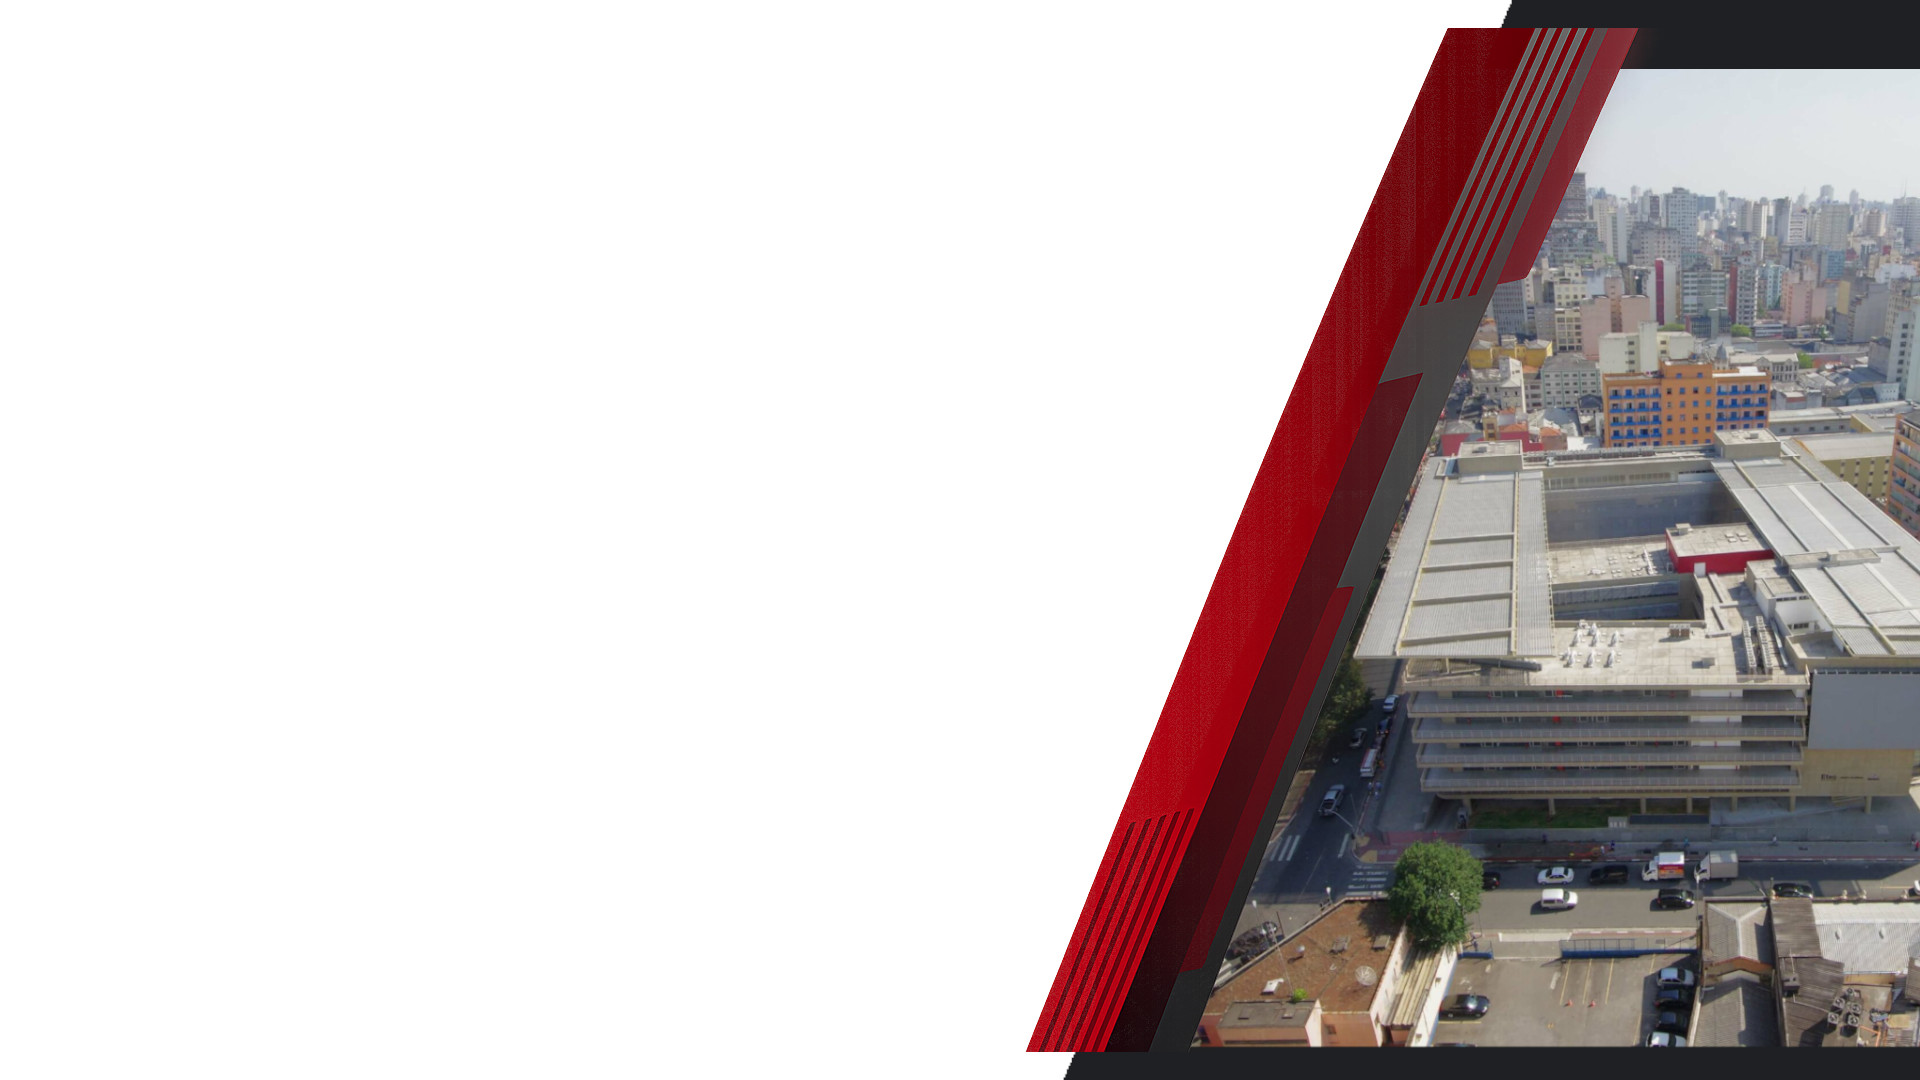
\includegraphics[width=\paperwidth,height=\paperheight]{imgs/img_001.jpg}%
}
\begin{frame}[b]{Pitch}
  \begin{itemize}
    \item \parbox{0.60\textwidth}{\textbf{O que é:} Solução tecnológica voltada para automação e monitoramento das plantações de mandioca}
    \item \parbox{0.60\textwidth}{\textbf{O problema:} Verificações manuais geram atrasos na detecção de falhas e desperdício de recursos}
    \item \parbox{0.60\textwidth}{\textbf{Proposta de valor:} Transformar dados coletados no campo em informações úteis e alertas em tempo hábil}
    \item \parbox{0.60\textwidth}{\textbf{Público-alvo:} Agricultores e responsáveis pelo gerenciamento de lavouras de mandioca}
    \item \parbox{0.60\textwidth}{\textbf{Tecnologia:} Sensores de campo, rede sem fio, servidor central, banco de dados e interface web}
  \end{itemize}
  
  \vfill
  
  {\fontsize{4}{5}\selectfont\textit{Fonte: Autores}\hfill\textcolor{white}{Imagem: Ilustração do projeto}}
\end{frame}
}

\section{Problematização}
{
\usebackgroundtemplate{%
  
\includegraphics[width=\paperwidth,height=\paperheight]{imgs/img_002.jpg}%
}
\begin{frame}[b]{Problematização}
  \begin{itemize}
    \item \parbox{0.60\textwidth}{\textbf{Acompanhamento manual:} Exige alto esforço operacional e não garante monitoramento contínuo}
    \item \parbox{0.60\textwidth}{\textbf{Detecção tardia:} Dificuldade para identificar alterações climáticas e do solo rapidamente}
    \item \parbox{0.60\textwidth}{\textbf{Desperdício de recursos:} Falta de precisão no manejo compromete insumos e produtividade}
    \item \parbox{0.60\textwidth}{\textbf{Ausência de histórico:} Inexistência de registros estruturados impede análises comparativas}
    \item \parbox{0.60\textwidth}{\textbf{Demora nas decisões:} Sem dados centralizados, a resposta a situações críticas torna-se lenta}
  \end{itemize}
  
  \vfill
  
  {\fontsize{4}{5}\selectfont\textit{Fonte: Autores}\hfill\textcolor{white}{Imagem: Desafios no campo}}
\end{frame}
}

\section{Estado da Arte}
\begin{frame}[t]{Estado da Arte}
  \scriptsize
  
  Análise de \textbf{soluções aplicadas à agricultura inteligente}, comparando abordagens de monitoramento remoto, automação agrícola e suporte à decisão para culturas como a mandioca.
  
  \vspace{0.3cm}
  
  \begin{table}
    \centering
    \tiny
    \begin{tabular}{|p{2.4cm}|p{2.0cm}|p{2.1cm}|p{2.0cm}|p{2.0cm}|p{1.6cm}|}
      \hline
      \textbf{Título/Autores} & \textbf{Objetivo} & \textbf{Método} & \textbf{Resultados} & \textbf{Limitações} & \textbf{Gap} \\
      \hline
      Monitoramento de umidade do solo com IoT — Santos et al. (2023) & Automatizar leitura hídrica em pequenas lavouras & Rede de sensores sem fio com envio para nuvem & Redução no tempo de inspeção manual & Foco restrito apenas à umidade do solo & Não integra múltiplas variáveis ambientais \\
      \hline
      Agricultura de precisão na mandiocultura — Silva e Costa (2022) & Avaliar impacto de variáveis ambientais no cultivo & Coleta periódica de solo, clima e luminosidade & Maior controle do desenvolvimento radicular & Registro feito de forma semiautomática & Ausência de alertas em tempo real ao produtor \\
      \hline
      Sistemas de apoio à decisão agrícola — Oliveira et al. (2024) & Centralizar dados de campo em dashboards web & Arquitetura cliente-servidor com banco relacional & Melhoria na organização do histórico produtivo & Interfaces complexas para pequenos produtores & Falta de solução dedicada à mandioca \\
      \hline
    \end{tabular}
  \end{table}
\end{frame}

\section{Objetivo}
{
\usebackgroundtemplate{%
  
\includegraphics[width=\paperwidth,height=\paperheight]{imgs/img_004.jpg}%
}
\begin{frame}[b]{Objetivo}
  \begin{itemize}
    \item \parbox{0.60\textwidth}{\textbf{Objetivo geral:} Desenvolver uma solução inteligente de monitoramento e automatização para plantações de mandioca}
    \item \parbox{0.60\textwidth}{\textbf{Objetivos específicos:}}
    \begin{itemize}
      \item \parbox{0.55\textwidth}{Monitorar condições do solo e do ambiente automaticamente}
      \item \parbox{0.55\textwidth}{Transmitir e armazenar dados históricos de forma segura}
      \item \parbox{0.55\textwidth}{Emitir alertas quando situações críticas forem detectadas}
    \end{itemize}
    \item \parbox{0.60\textwidth}{\textbf{Entrega esperada:} Sistema integrado de coleta, armazenamento e visualização}
    \item \parbox{0.60\textwidth}{\textbf{Meta de impacto:} Reduzir processos manuais e agilizar a tomada de decisão}
  \end{itemize}
  
  \vfill
  
  {\fontsize{4}{5}\selectfont\textit{Fonte: Autores}\hfill\textcolor{white}{Imagem: Objetivos do sistema}}
\end{frame}
}

\section{Arquitetura e Ferramental}
{
\usebackgroundtemplate{%
  
\includegraphics[width=\paperwidth,height=\paperheight]{imgs/img_005.jpg}%
}
\begin{frame}[b]{Arquitetura e Ferramental (Conceitual)}
  \begin{itemize}
    \item \parbox{0.60\textwidth}{\textbf{Sensores de Campo:} Umidade do solo, temperatura, umidade do ar e luminosidade}
    \item \parbox{0.60\textwidth}{\textbf{Sistema de Rede:} Conexão sem fio dos sensores até o \textit{gateway} e envio ao servidor}
    \item \parbox{0.60\textwidth}{\textbf{Servidor / Backend:} Recebimento, processamento de regras e disparo de alertas}
    \item \parbox{0.60\textwidth}{\textbf{Banco de Dados:} Modelagem relacional para responsáveis, sensores, leituras e alertas}
    \item \parbox{0.60\textwidth}{\textbf{Interface / Dashboard:} Aplicação web para consulta em computador e dispositivos}
  \end{itemize}
  
  \vfill
  
  {\fontsize{4}{5}\selectfont\textit{Fonte: Autores}\hfill\textcolor{white}{Imagem: Componentes tecnológicos}}
\end{frame}
}

\section{Metodologia}
{
\usebackgroundtemplate{%
  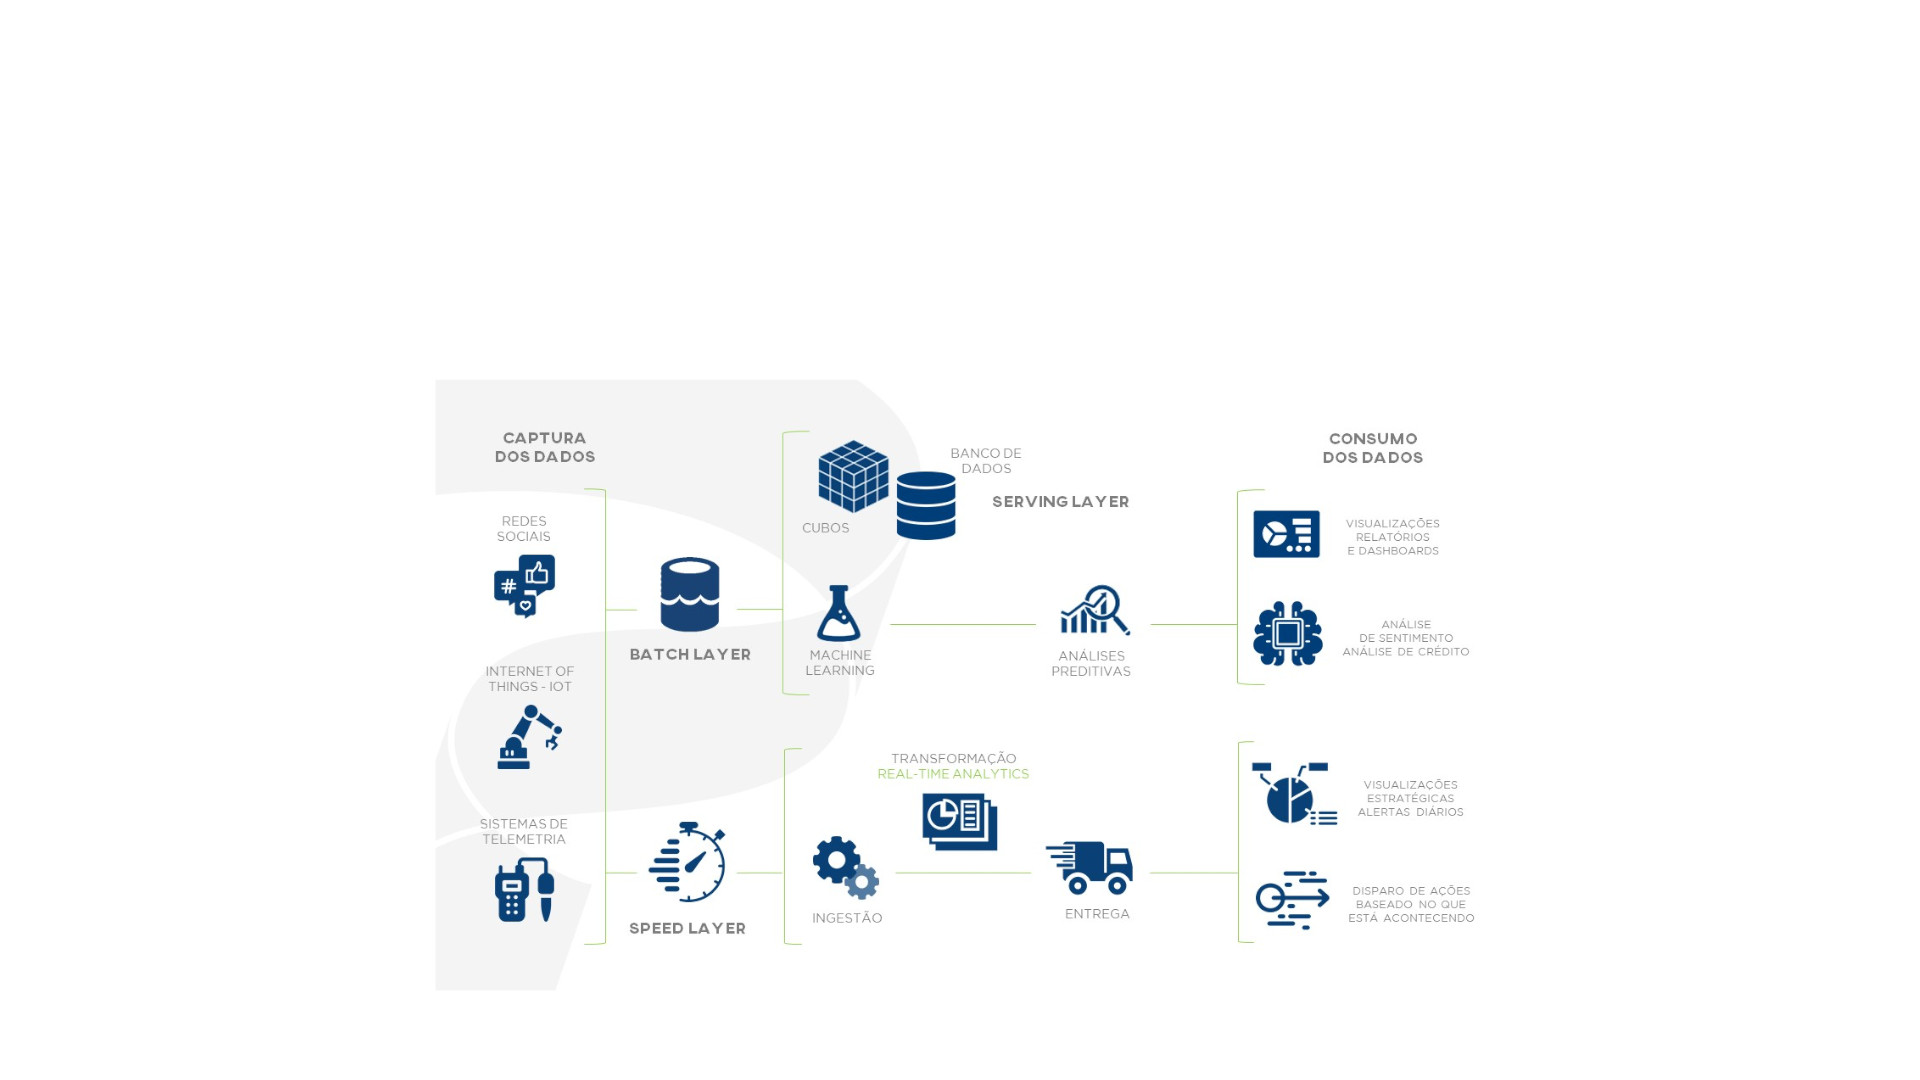
\includegraphics[width=\paperwidth,height=\paperheight]{imgs/img_006.jpg}%
}
\begin{frame}[t]{Metodologia — Fluxo da Solução}
  \scriptsize
  A arquitetura da \textbf{AutoMandi} integra a coleta física na plantação ao processamento digital, garantindo que o agricultor receba informações estruturadas e alertas em tempo hábil:

  \vspace{0.6cm}

  \begin{center}
  \begin{tikzpicture}[
    node distance=0.35cm and 0.45cm,
    box/.style={
      rectangle,
      rounded corners=3pt,
      draw=azulComplementar,
      fill=white,
      line width=1pt,
      text width=1.85cm,
      minimum height=1.0cm,
      align=center,
      font=\tiny\bfseries
    },
    highlight/.style={
      rectangle,
      rounded corners=3pt,
      draw=vermelhoPrincipal,
      fill=vermelhoPrincipal!10,
      line width=1.2pt,
      text width=1.85cm,
      minimum height=1.0cm,
      align=center,
      font=\tiny\bfseries
    },
    arrow/.style={
      -{Stealth[length=2mm]},
      thick,
      color=vermelhoPrincipal
    }
  ]

    % Linha 1: Coleta e Transmissão
    \node[box] (plantacao) {1. Plantação\\{\normalfont\tiny Ambiente agrícola}};
    \node[highlight, right=of plantacao] (sensores) {2. Sensores\\{\normalfont\tiny Solo, clima e luz}};
    \node[box, right=of sensores] (rede) {3. Rede / Gateway\\{\normalfont\tiny Conexão sem fio}};
    \node[highlight, right=of rede] (servidor) {4. Sistema / Servidor\\{\normalfont\tiny Processamento}};

    % Linha 2: Armazenamento e Visualização
    \node[box, below=0.8cm of servidor] (banco) {5. Banco de Dados\\{\normalfont\tiny Histórico e alertas}};
    \node[highlight, left=of banco] (dashboard) {6. Dashboard\\{\normalfont\tiny Interface visual}};
    \node[box, left=of dashboard] (usuario) {7. Agricultor\\{\normalfont\tiny Tomada de decisão}};

    % Setas
    \draw[arrow] (plantacao) -- (sensores);
    \draw[arrow] (sensores) -- (rede);
    \draw[arrow] (rede) -- (servidor);
    \draw[arrow] (servidor) -- (banco);
    \draw[arrow] (banco) -- (dashboard);
    \draw[arrow] (dashboard) -- (usuario);

  \end{tikzpicture}
  \end{center}
\end{frame}
}

\section{Funcionalidades do Sistema}
{
\usebackgroundtemplate{%
  
\includegraphics[width=\paperwidth,height=\paperheight]{imgs/img_007.jpg}%
}
\begin{frame}[b]{Funcionalidades do Sistema}
  \begin{itemize}
    \item \parbox{0.60\textwidth}{\textbf{Monitorar Plantação:} Acompanhamento contínuo dos dados coletados pelos sensores}
    \item \parbox{0.60\textwidth}{\textbf{Registrar Dados:} Armazenamento estruturado das leituras para consultas futuras}
    \item \parbox{0.60\textwidth}{\textbf{Gerar Alertas:} Identificação automática de condições que exigem atenção imediata}
    \item \parbox{0.60\textwidth}{\textbf{Exibir Histórico:} Consulta de registros anteriores para análise da evolução da lavoura}
    \item \parbox{0.60\textwidth}{\textbf{Gerenciar Usuários e Visualização:} Controle de acesso e apresentação organizada via aplicação}
  \end{itemize}
  
  \vfill
  
  {\fontsize{4}{5}\selectfont\textit{Fonte: Autores}\hfill\textcolor{white}{Imagem: Funcionalidades da plataforma}}
\end{frame}
}

\section{Benefícios Esperados e Conclusão}
{
\usebackgroundtemplate{%
  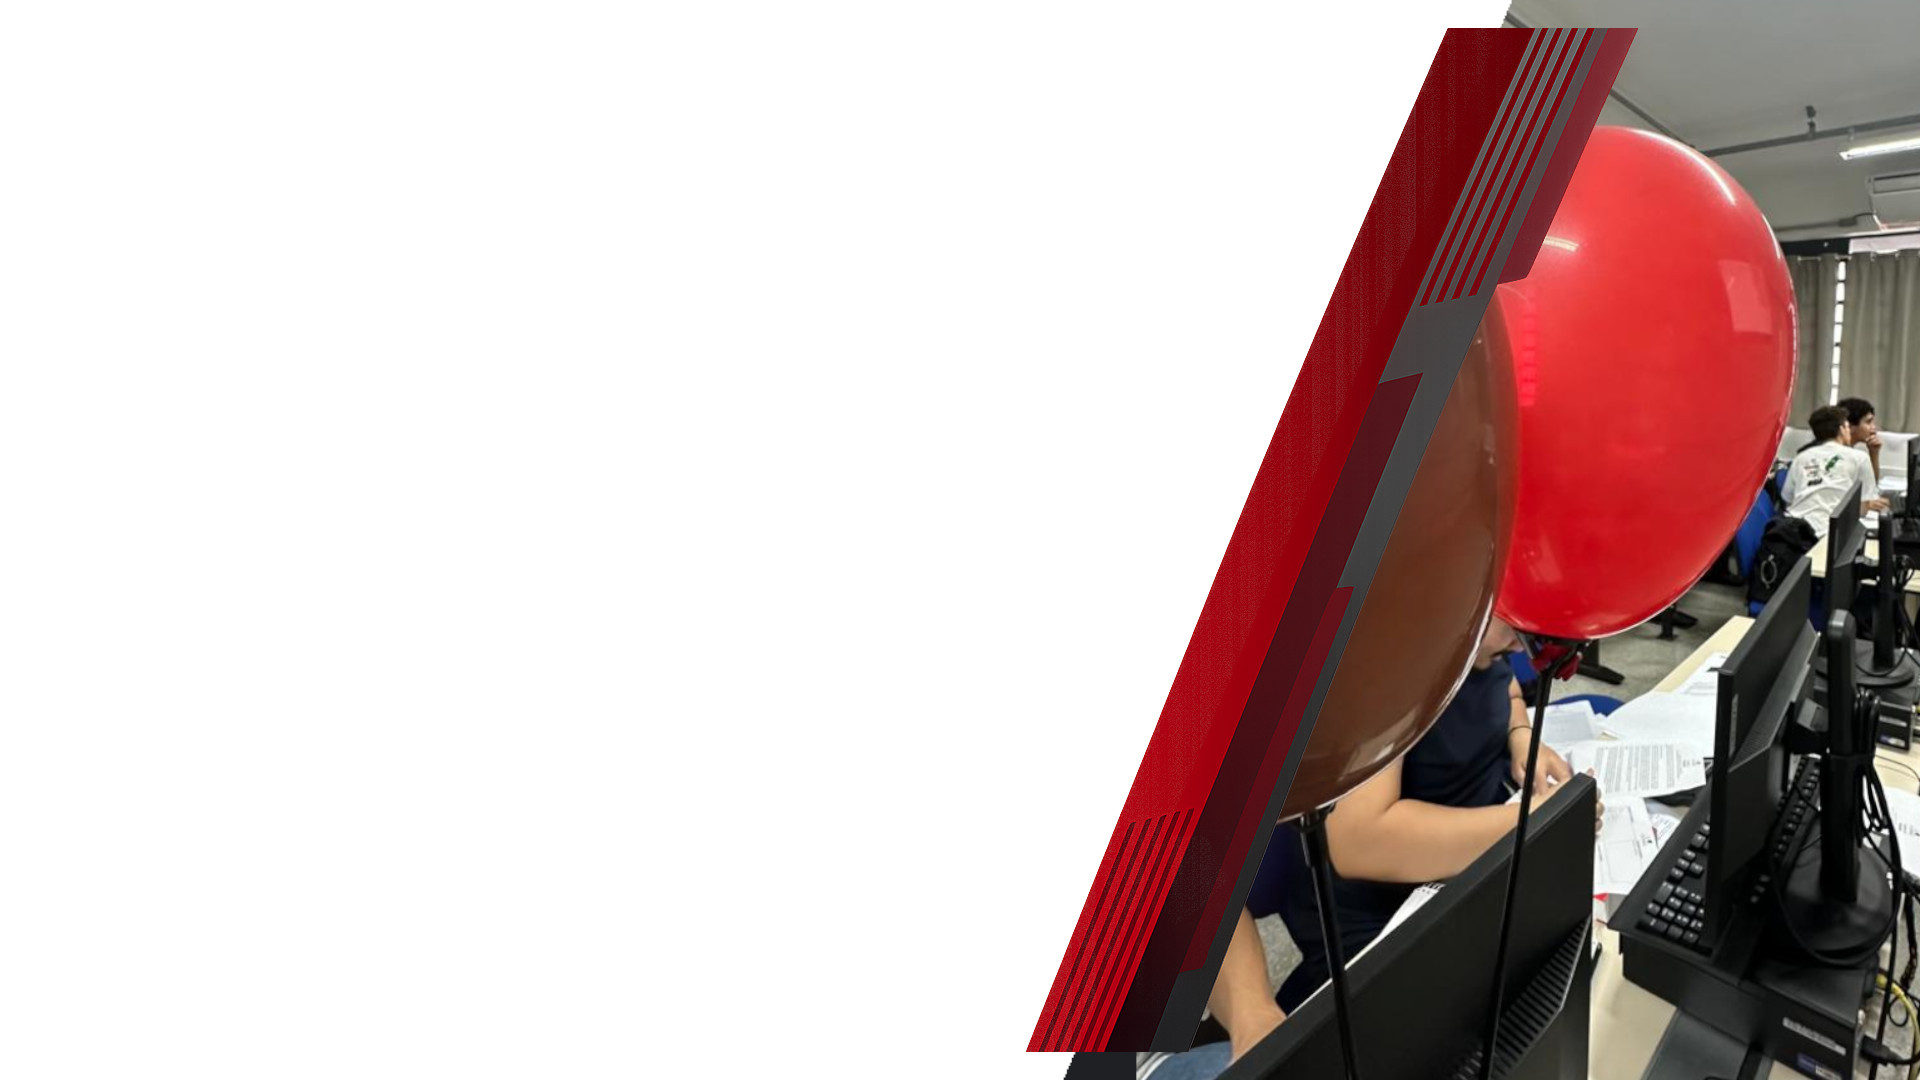
\includegraphics[width=\paperwidth,height=\paperheight]{imgs/img_008.jpg}%
}
\begin{frame}[b]{Benefícios Esperados e Conclusão}
  \begin{itemize}
    \item \parbox{0.60\textwidth}{\textbf{Para a plantação:} Monitoramento eficiente, detecção rápida de alterações e controle ambiental}
    \item \parbox{0.60\textwidth}{\textbf{Para a operação:} Redução de desperdícios, otimização de recursos e automação de processos}
    \item \parbox{0.60\textwidth}{\textbf{Para o responsável:} Acesso centralizado ao histórico, recebimento de alertas e decisões ágeis}
    \item \parbox{0.60\textwidth}{\textbf{Conclusão:} A AutoMandi integra sensores, redes e banco de dados para modernizar o cultivo}
    \item \parbox{0.60\textwidth}{\textbf{Impacto:} Contribui para uma agricultura mais organizada, eficiente e inteligente}
  \end{itemize}
  
  \vfill
  
  {\fontsize{4}{5}\selectfont\textit{Fonte: Autores}\hfill\textcolor{white}{Imagem: Resultados esperados}}
\end{frame}
}

% Slide Final
{
\usebackgroundtemplate{%
  
\includegraphics[width=\paperwidth,height=\paperheight]{imgs/img_022.jpg}%
}
\begin{frame}[b]{}
  \vspace{0.2cm}
  
  \hspace*{0.25\paperwidth}{\Large \textbf{Obrigado!}}
  
  \vfill
\end{frame}
}

\end{document}